\documentclass{beamer}
% Load Packages
\usepackage[utf8]{inputenc}
\usepackage{xcolor}
\usepackage{tikz}
\usetikzlibrary{positioning,calc}
\usepackage[absolute,overlay]{textpos}
\usepackage{graphicx}
\usepackage{hyperref}
\usepackage{amsmath}
\usepackage{listings}
\usepackage{fontawesome}
\usepackage[brazilian]{babel}
\usepackage{datetime}
\usepackage{subcaption} % usado para figuras lado a lado

% Define Commands
\newcommand*{\ClipSep}{0.06cm} %To adjust footer logo
\newcommand{\E}{\mathrm{e}\,} %\def\I{e} % used to defined e for exp(x), see later what it should be
\newcommand{\ud}{\mathrm{d}}
\lstset{numbers=left, numberstyle=\tiny, stepnumber=1,firstnumber=1,breaklines=true,
    numbersep=5pt,language=Python,
    stringstyle=\ttfamily,
    basicstyle=\footnotesize, 
    showstringspaces=false
}
 
\usetheme{oxonian}
\setbeamertemplate{itemize subitem}{$-$}
\setbeamertemplate{itemize subsubitem}[circle]
\setbeamercolor{block body alerted}{bg=alerted text.fg!10}
\setbeamercolor{block title alerted}{bg=alerted text.fg!20}
\setbeamercolor{block body}{bg=structure!10}
\setbeamercolor{block title}{bg=structure!20}
\setbeamercolor{block body example}{bg=green!10}
\setbeamercolor{block title example}{bg=green!20}
\setbeamertemplate{blocks}[rounded][shadow]
 
\title{Introdução a Orientação a Objetos}
\subtitle{Programação Estruturada e Orientada a Objetos}
\titlegraphic{
\includegraphics[width=2.5cm]{Theme/Logos/ifrn_cm_vertical.png}}
\author{Prof. Me. Leo Moreira Silva}

\date{\today}

\begin{document}

{\setbeamertemplate{footline}{} 
\frame{\titlepage}}

\section*{Agenda}\begin{frame}{Agenda}\tableofcontents\end{frame}

\section{Introdução}

\begin{frame}{Introdução}
    \begin{itemize}
        \item Programas eram lineares e com poucos módulos (Programação Estruturada)
        \item Aumento da complexidade dos sistemas e difícil \textbf{reusabilidade} de componentes;
        \item Criou-se um novo paradigma para análise e desenvolvimento de sistemas: a \textbf{Programação Orientada a Objetos}.
    \end{itemize}
\end{frame}

\begin{frame}{Introdução}
    \begin{figure}
        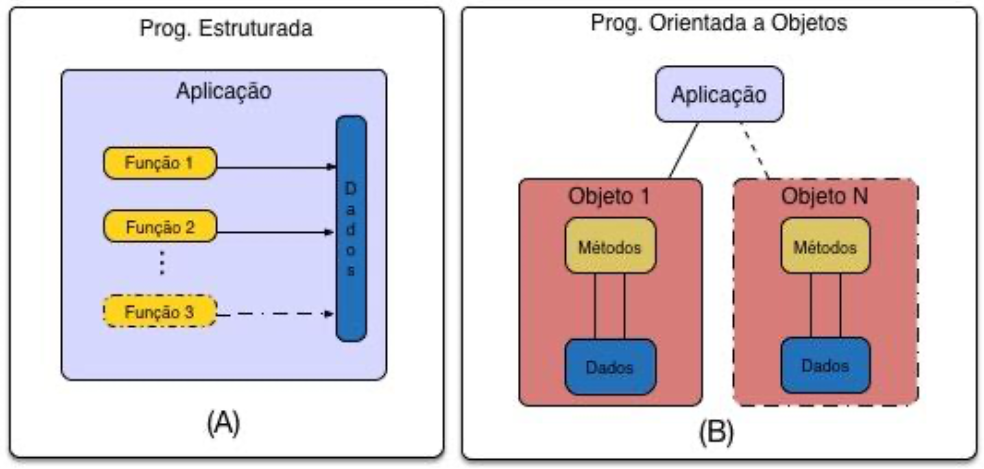
\includegraphics[width=10cm]{Theme/Logos/progest_x_progobj.png}
    \end{figure}
\end{frame}

\section{Paradigma da Orientação a Objetos}

\begin{frame}{Paradigma da Orientação a Objetos}
    \begin{itemize}
        \item O paradigma OO surgiu no fim dos anos 60
        \item Alan Kay, um dos pais desse paradigma, formulou a chamada analogia biológica:
        \begin{itemize}
            \item "Como seria um sistema de software que funcionasse como um ser vivo?"
        \end{itemize}
    \end{itemize}
    \begin{figure}
        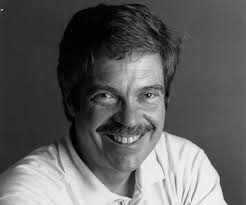
\includegraphics[width=3cm]{Theme/Logos/alan_kay.png}
    \end{figure}
\end{frame}

\begin{frame}{Analogia Biológica}
    \begin{itemize}
        \item Cada célula interagiria com outras células através do envio de mensagens para realizar um objetivo comum
        \item Adicionalmente, cada célula se comportaria como uma unidade autônoma
        \item De uma forma mais geral, Alan Kay pensou em como construir um sistema de software a partir de \textbf{agentes autônomos} que \textbf{interagem entre si}.
    \end{itemize}
    \begin{figure}
        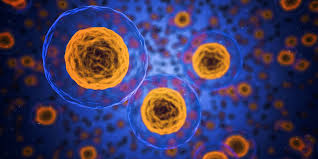
\includegraphics[width=4cm]{Theme/Logos/celula.png}
    \end{figure}
\end{frame}

\section{Fundamentos da Orientação a Objetos}

\begin{frame}{Fundamentos da Orientação a Objetos}
    \begin{itemize}
        \item Através de sua analogia biológica, Alan Kay definiu os fundamentos da orientação a objetos:
        \begin{enumerate}
            \item Qualquer coisa é um objeto
            \item Objetos realizam tarefas através da requisição de serviços a outros objetos
            \item Cada objeto pertence a uma determinada classe. Uma classe agrupa objetos similares
            \item A classe é um repositório para comportamento associado ao objeto
            \item Classes são organizadas em hierarquias
        \end{enumerate}
    \end{itemize}
\end{frame}

\begin{frame}{SSOO: uma analogia}
    \begin{figure}
        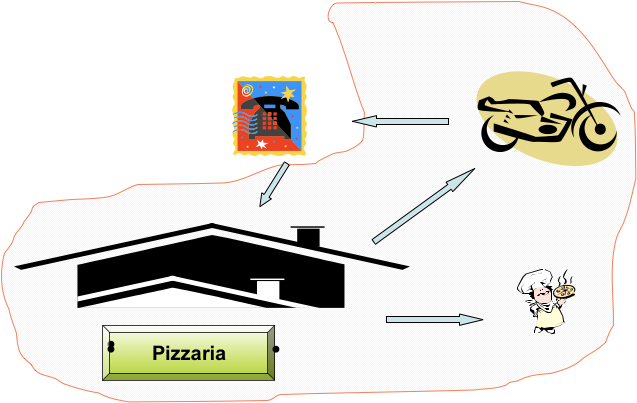
\includegraphics[width=10cm]{Theme/Logos/exemplo_ssoo.png}
    \end{figure}
\end{frame}

\section{Conceitos da Orientação a Objetos}

\begin{frame}{Conceitos da Orientação a Objetos}
    \begin{itemize}
        \item Conceitos:
        \begin{itemize}
            \item Objeto
            \item Classe
            \item Instância
        \end{itemize}
    \end{itemize}
\end{frame}

\begin{frame}{Objeto}
    \begin{itemize}
        \item Entidade concretas ou abstratas
        \item Tem características e podem executar ações;
        \item "Um objeto representa um item identificável, uma unidade ou entidade, individual, seja real ou abstrato, com uma regra bem definida":
        \begin{block}{}
            Objeto = dados + operações
        \end{block}
        \item Possuem:
        \begin{itemize}
            \item Estado
            \item Comportamento
            \item Identidade
        \end{itemize}
    \end{itemize}
\end{frame}

\begin{frame}{Objeto}
    \begin{itemize}
        \item Estado:
        \begin{itemize}
            \item Define os estados possíveis que um objeto pode assumir
            \item São os valores dos \textbf{atributos} (propriedades)
        \end{itemize}
        \item Exemplo:
    \end{itemize}
    \begin{figure}[H]
        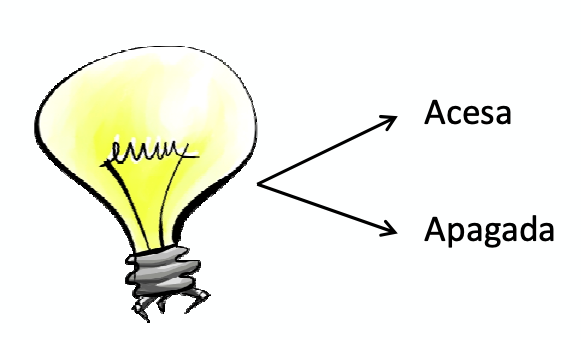
\includegraphics[width=5cm]{Theme/Logos/estado_lampada.png}
    \end{figure}
\end{frame}

\begin{frame}{Objeto}
    \begin{itemize}
        \item Comportamento:
        \begin{itemize}
            \item São as funções que podem ser executadas por um determinado objeto
            \item Corresponde aos \textbf{métodos}
            \item O que se pode fazer com o objeto
        \end{itemize}
        \item Exemplo:
    \end{itemize}
    \begin{figure}[H]
        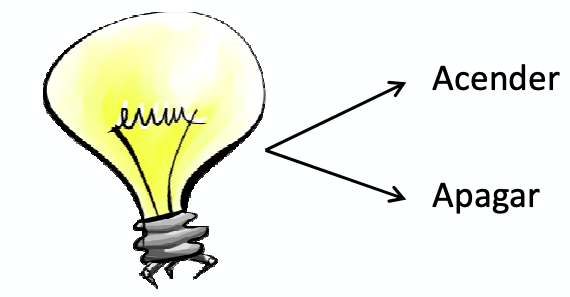
\includegraphics[width=5cm]{Theme/Logos/lampada_comportamento.png}
    \end{figure}
\end{frame}

\begin{frame}{Objeto}
    \begin{itemize}
        \item Identidade:
        \begin{itemize}
            \item Um objeto é único, mesmo que o seu estado seja idêntico ao de outro.
        \end{itemize}
        \item Exemplo:
    \end{itemize}
    \begin{figure}[H]
        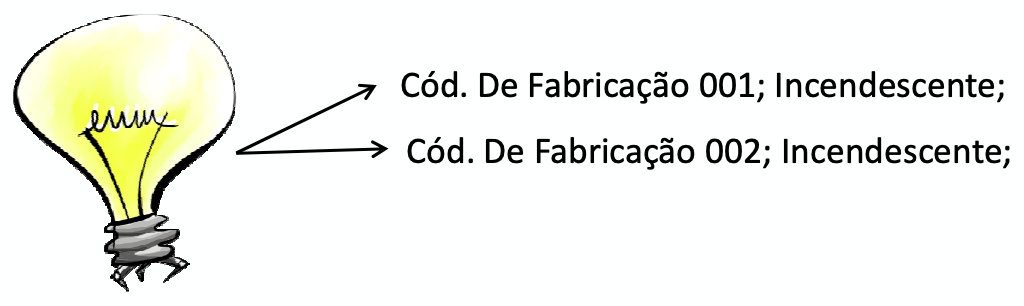
\includegraphics[width=8cm]{Theme/Logos/lampada_identidade.png}
    \end{figure}
\end{frame}

\begin{frame}{Classe}
    \begin{itemize}
        \item Modelo ou esquema a partir do qual os objetos são criados (instanciados)
        \item Modelam os objetos, definindo:
        \begin{itemize}
            \item Tipos de dados que o objeto armazena, ou seja, os estados possíveis que ele pode assumir (\textbf{atributos})
            \item Tipos de operações que podem ser executadas pelo objeto, ou seja, o seu comportamento (\textbf{métodos})
        \end{itemize}
        \item Abstração de objetos de características semelhantes
        \item É a \textbf{essência} do objeto
    \end{itemize}
\end{frame}

\begin{frame}{Classe}
    \begin{itemize}
        \item Objetos são instâncias de classes:
        \begin{figure}[H]
            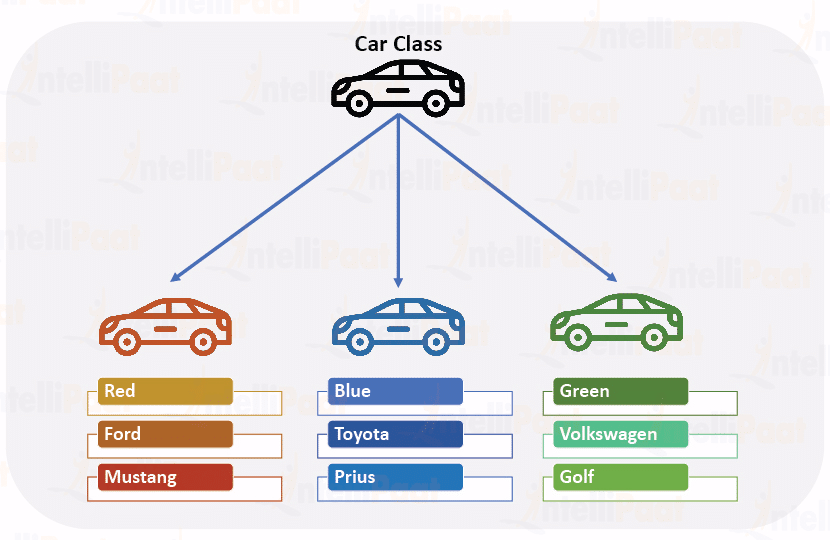
\includegraphics[width=9cm]{Theme/Logos/exemplo_classe_instancia.png}
        \end{figure}
    \end{itemize}
\end{frame}

\begin{frame}{Classe}
    \begin{itemize}
        \item Objetos são instâncias de classes:
        \begin{figure}[H]
            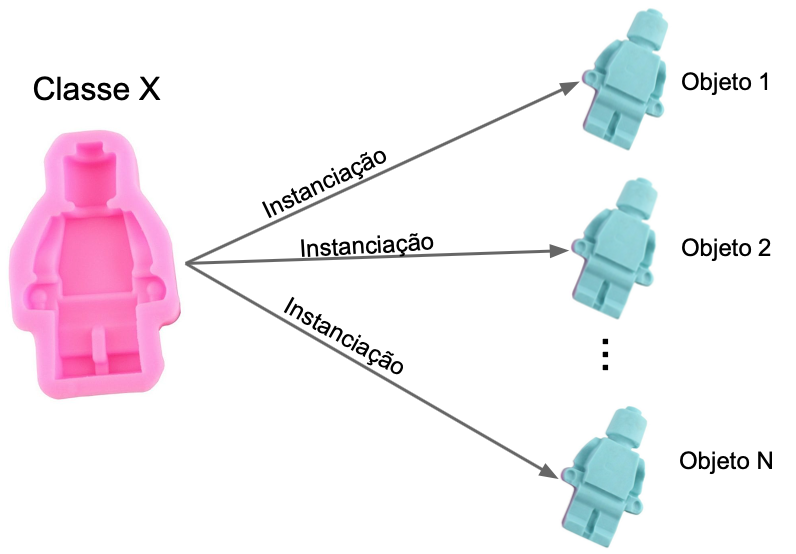
\includegraphics[width=9cm]{Theme/Logos/exemplo2_classe_instancia.png}
        \end{figure}
    \end{itemize}
\end{frame}

\begin{frame}{Classe}
    \large
    \begin{block}{Importante}
        Todo código Orientado a Objeto está dentro de uma classe!
    \end{block}
\end{frame}

\begin{frame}{Classe}
    \begin{itemize}
        \item Classe:
    \end{itemize}
    \begin{figure}[H]
        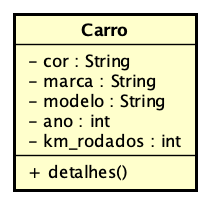
\includegraphics[width=3.5cm]{Theme/Logos/classe_carro.png}
    \end{figure}
\end{frame}

\begin{frame}[fragile]{Classe}
    \begin{itemize}
        \item Definindo classe em Python:
    \end{itemize}
    \begin{semiverbatim}
        class NomeClasse:
            atributo_1 = valor_1
            atributo_2 = valor_2
            atributo_3 = valor_3
        def metodo_1(self):
            #faz algo aqui
    \end{semiverbatim}
    \begin{itemize}
        \item Uma nova instância pode ser criada a partir da chamada:
        \begin{semiverbatim}
            variavel = NomeClasse()
        \end{semiverbatim}
        \item 'variavel' irá armazenar a instância criada
    \end{itemize}
\end{frame}

\begin{frame}{Classe}
    \begin{itemize}
        \item \texttt{self} é uma variável que referencia um determinado objeto da classe
        \item Todo método de uma classe recebe \texttt{self} como primeiro parâmetro
        \item Tal parâmetro indica qual objeto está executando aquele método
        \item \texttt{self} deve preceder um atributo da classe dentro de métodos
    \end{itemize}
\end{frame}

\begin{frame}[fragile]{Classe}
\small
\begin{semiverbatim}
class Carro:
    cor = 'sem cor'
    marca = 'sem marca'
    modelo = 'sem modelo'
    ano = 2010
    km_rodados = 0

    def detalhes(self):
        print 'cor:', self.cor
        print 'marca:', self.marca
        print 'modelo:', self.modelo
        print 'ano:', self.ano
        print 'km rodados:', self.km_rodados
\end{semiverbatim}
\end{frame}

\begin{frame}[fragile]{Classe}
\scriptsize
\begin{semiverbatim}
>>>car_1 = Carro() #Instancia o objeto da classe Carro na variável 'car_1'
>>>car_1.cor = 'Vermelho'
>>>car_1.marca = 'Honda'
>>>car_1.modelo = 'HR-V'
>>>car_1.ano = 2016
>>>car_1.detalhes() #Chama o método 'detalhes' implementado na classe Carro

cor: Vermelho
marca: Honda
modelo: HR-V
ano: 2016
km_rodados: 0
\end{semiverbatim}
\end{frame}

\begin{frame}{Classe}
    \begin{figure}[H]
        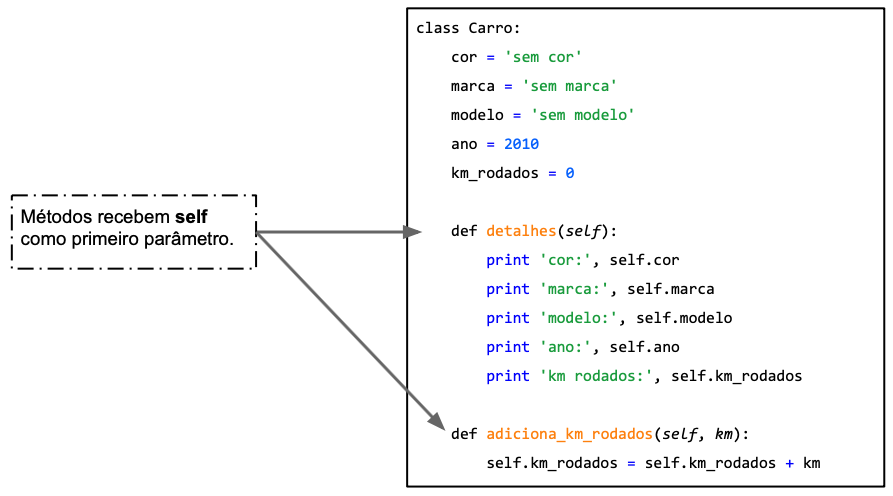
\includegraphics[width=10cm]{Theme/Logos/self_1.png}
    \end{figure}
\end{frame}

\begin{frame}{Classe}
    \begin{figure}[H]
        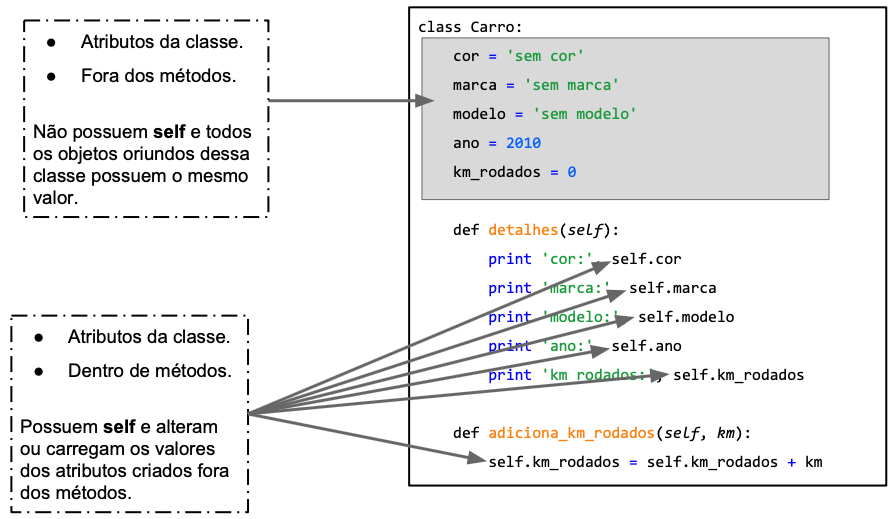
\includegraphics[width=10cm]{Theme/Logos/self_2.png}
    \end{figure}
\end{frame}

\begin{frame}{Classe}
    \begin{figure}[H]
        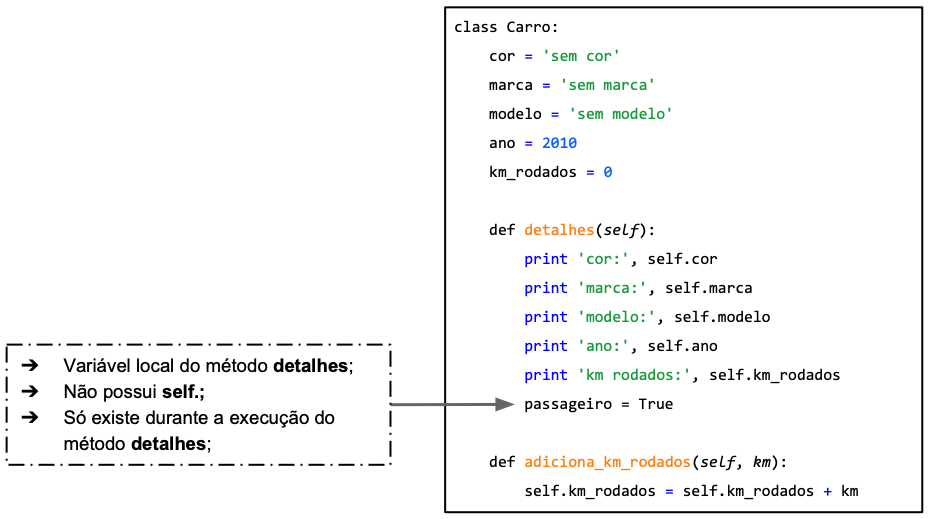
\includegraphics[width=10cm]{Theme/Logos/self_3.png}
    \end{figure}
\end{frame}

\begin{frame}{Dúvidas?}
    \begin{figure}
        
\includegraphics[scale=0.35]{Theme/Logos/duvidas_frequentes.png}
    \end{figure}
\end{frame}

\section{Exercícios}

\begin{frame}{Exercício 1}
    \begin{enumerate}
        \item Copiar o código da classe Carro
        \item Criar um novo objeto, com valores diferentes do slide
        \item Imprimir os dados
        \item Criar e implementar um novo método chamado \texttt{diminuir\_km\_rodados()}
        \item Testar o método criado
    \end{enumerate}
\end{frame}

\begin{frame}{Exercício 1 (Cont.)}
    \begin{enumerate}
        \item Implementar os métodos abaixo
        \begin{enumerate}
            \item ligarMotor
            \item desligarMotor
        \end{enumerate}
        \item Criar atributo para:
        \begin{enumerate}
            \item estado do motor (ligado/desligado)
        \end{enumerate}
    \end{enumerate}
\end{frame}

\begin{frame}{Exercício 2}
    \begin{enumerate}
        \item Implementar e testar a seguinte classe:
    \end{enumerate}
    \begin{figure}[H]
        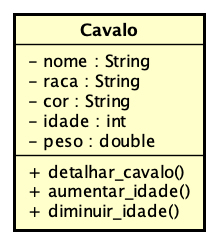
\includegraphics[width=3.5cm]{Theme/Logos/classe_cavalo.png}
    \end{figure}
\end{frame}

\end{document}